\documentclass[a4paper,11pt]{article}
\usepackage{adjustbox}
\usepackage[affil-it]{authblk}
\usepackage{amsmath}
\usepackage{amsfonts}   % if you want the fonts
\usepackage{amssymb}    % if you want extra symbols
\usepackage{bm}
\usepackage{etoolbox}
\usepackage{float}
\usepackage[hang,flushmargin,bottom]{footmisc} % footnote format
\usepackage[hidelinks]{hyperref} % hyperref package & removing outline from links
\usepackage{graphicx}   % need for figures	
\usepackage[margin=1in]{geometry}	
\usepackage{lmodern}
%\usepackage{mathptmx}
\usepackage{multicol}
\usepackage{physics}
\usepackage{rotating}
\usepackage{secdot}
\usepackage{siunitx} % Formats the units and values
\usepackage{tabulary}
%\usepackage{tablefootnote}
\usepackage{textcomp}
\usepackage{tikz}
\usepackage{titlesec}
\usepackage{titling}
\usepackage[utf8]{inputenc}
\usepackage{xcolor}

\usepackage[numbers,sort&compress]{natbib} % format bibliography
\renewcommand{\bibsection}{}
\setlength{\bibsep}{0.0pt}

\makeatletter
\patchcmd{\@maketitle}{\LARGE \@title}{\fontsize{18}{8.5}\selectfont\@title}{}{}
\makeatother


\renewcommand\Authfont{\fontsize{11}{1}\selectfont}
\renewcommand\Affilfont{\fontsize{11}{1}\itshape}


\titleformat*{\section}{\large\bfseries}

\title{\vspace{-2.0cm}\textbf{Measurement of Drag Coefficients through Vegetation Canopy} }
\author{Ryan Falkenstein-Smith, Kevin McGrattan, Blaza Toman, and Marco Fernandez}
\affil{National Institute of Standards and Technology}
\date{\vspace{-5ex}}

\begin{document}

\maketitle
\thispagestyle{empty}

\section{Introduction}
The Fire Dynamic Simulator (FDS)~\cite{FDS_Tech_Guide}, has recently been extended to model fires in the wildland-urban interface (WUI). A crucial component of this model is a clear depiction of wind-driven flow through vegetation. There have been several drag coefficient measurements of vegetation~\cite{Cao2012,Jalonen2014,Mayhead1973} that places a single plant or small tree within a wind-tunnel wherein the resistance force is measured. The measurement, however, isn’t necessarily translatable to a CFD model which could consider the vegetation structure as a collection of subgrid-scale objects that decrease the momentum of the flowing gases. In this work, the drag coefficients through different vegetation canopies are measured within a wind-tunnel to complement local conditions applied in CFD models.

\section{Experimental Method}
Vegetation that occupies a grid cell is typically modeled as a collection of subgrid-scale Lagrangian particles whose mass, size, and shape are characterized by a handful of parameters that can be determined from field measurements. Previous works have established configurations that better describe the force exerted per unit volume in vegetation~\cite{Mueller2014}. In this work, the drag force is defined as:
\begin{equation}\label{eq:Pressure}
F \equiv \frac{\Delta P}{L}  = \frac{\rho}{2} \, C_{\rm d} \, \kappa \, U^2
\end{equation}
where $\frac{\Delta P}{L}$ is the pressure drop per unit length, $U$ is an average flow speed, $\rho$ is the gas density, $C_{d}$ is the drag coefficient taken as a constant. The parameter $\kappa$ resembles an absorption coefficient that combines the volume fraction, shape factor, and surface to volume ratio of the vegetation. The parameter $\kappa$ can be determined by measuring the projected area of light passing a distance L through the vegetation. The relative area of light, or “free-area coefficient,” is defined by the relation: 
\begin{equation}\label{eq:WhiteFraction}
W = {\rm e}^{-\kappa L}
\end{equation}

A variety of vegetation species with different leaf shapes (i.e., needle, elliptic, scale, and ovate) was chosen for this study based on local availability. Vegetation samples were cut into 0.5 \si{m} by 0.5 \si{m} by 0.5 \si{m} cubes to occupy the cross-section of the wind-tunnel fully. Vegetation samples were reoriented relative to the flow and pruned to generate multiple vegetation configurations using the same vegetation species. The parameter $\kappa$ was obtained by photographing the projected area of each vegetation configuration against a white backdrop. The images were processed using MATLAB’s Image Processing Toolbox to determine the free-are coefficient of the vegetation, $W$. Once obtained, the free area coefficient was used to calculate $\kappa$ from Eq.~ref{}.

As shown in Fig.~\ref{fig:WindtunnelPic}’s schematic diagram, pressure loss and air flow measurements were measured simultaneously using an MKS Baratron Type 220D pressure transducer and a Rosemont 485 Annubar, respectively. Air density was calculated from the pressure and temperature readings of the testing facility. Each test consisted of taking pressure loss and flow measurements across nine different fan speeds ranging from 0 to 88\% of the full-scale fans speed. Tests were repeated three times for each sample configuration and compared to determine the variance homogeneity the repeated measurements. 

\begin{figure} [!]
	\centering 	
    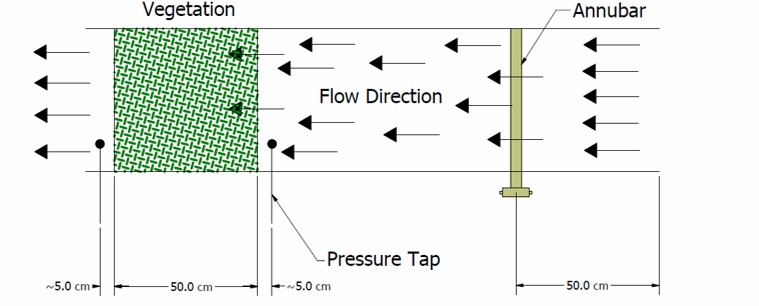
\includegraphics[width=\textwidth,keepaspectratio]{Picture6a.jpg}
	\caption[Wind tunnel experimental setup]{Wind tunnel experimental setup with top and front schematic drawings }
	\label{fig:WindtunnelPic}
\end{figure}

\section{Results}
The average drag coefficient of all sample configurations was determined to be 2.8 with an expanded uncertainty of 0.4. A random-effects one-way ANOVA was implemented on the drag coefficients of different vegetation samples. The analysis yielded a significant variation among the species. Further examination using a Tukey’s test, showed only a single difference between vegetation two species. Despite the significant difference, the average drag coefficient of each species was still within the uncertainty bounds of the overall average drag coefficient, suggesting that the significant difference may not be large enough to have a practical implication. 

\section{Conclusion}
The primary objective of this work was to calculate the drag coefficients of bulk vegetation to be incorporated into CFD models. It was found that the overall average drag coefficient of the bulk vegetation was found to be 2.8 with an expanded uncertainty of 0.4. Although some difference in average drag coefficients was observed between different species, they may not be large enough to have practical implications, indicating that the overall average drag coefficient could be used as a constant value in CFD models of various plant types.

\section*{References}
\addcontentsline{toc}{section}{References}
\bibliographystyle{unsrt}
\bibliography{References}
\end{document}
